\documentclass[a4paper,12pt, english]{article}
\usepackage[a4paper, left=2.5cm, right=2cm, top=2.3cm, bottom=3cm]{geometry} % kleinere Ränder
\usepackage[singlespacing]{setspace}
\usepackage{comment} % Zum Auskommentieren ganzer Codeblöcke
\usepackage{fancyhdr}
\pagestyle{fancy}
\fancyhf{}
%\fancyhead[R]{\itshape \leftmark}
\cfoot{\thepage}

%% commenting macros

% use this to hide larger blocks of material:
\usepackage{xcolor}
\usepackage{amsmath,amssymb}

% Define colors for authors
\definecolor{johannescolor}{rgb}{0.2,0.6,0.6}
\definecolor{danjecolor}{rgb}{0,0.7,0}

% Define colors for general macros
\definecolor{todocolor}{rgb}{0.9,0.1,0.1}
\definecolor{changedcolor}{rgb}{0.42,0.27,0.57}
\definecolor{addedcolor}{rgb}{0.867,0.176,0.361}
\definecolor{sourcecolor}{rgb}{0.25,0.4,0.7}

% General comment macro
\newcommand{\nbc}[3]{
    {\colorbox{#3}{\bfseries\sffamily\scriptsize\textcolor{white}{#1}}}
    {\textcolor{#3}{\sf\small$\blacktriangleright$\textit{#2}$\blacktriangleleft$}}
}
\newcommand{\cbs}[3]{
    {\colorbox{#2}{\bfseries\sffamily\scriptsize\textcolor{white}{#1}}}
}
  
% Define individual comments for authors
\newcommand{\johannes}[1]{\nbc{Johannes}{#1}{johannescolor}}
\newcommand{\danje}[1]{\nbc{Danje}{#1}{danjecolor}}

% Define general helper macros
\newcommand{\todo}[1]{\nbc{TODO}{#1}{todocolor}}
\newcommand{\changed}[1]{\nbc{CHANGED}{#1}{changedcolor}}
\newcommand{\added}[1]{\nbc{ADDED}{#1}{addedcolor}}
\newcommand{\source}[1]{\cbs{SOURCE MISSING}{sourcecolor}}

\newcommand{\redacted}[1]{\emph{[anonymized for review]}}
%\renewcommand{\redacted}[1]{#1}

% Use this to temporarily hide reviewing comments, todos, etc.:
%  \renewcommand{\jane}[1]{}
%  \renewcommand{\john}[1]{}

% Use this to make "changed" items appear normal:
%\renewcommand{\changed}[1]{#1}
%\renewcommand{\added}[1]{#1}
%\renewcommand{\todo}[1]{}

%% end commenting macros

% Umlaute in der Datei erlauben, auf deutsch umstellen
\usepackage[utf8]{inputenc}
%\usepackage[ngerman]{babel}
\usepackage[nottoc,numbib]{tocbibind}
%\usepackage{mathptmx} % Hier steckt Times drin
%\usepackage{fontspec}
%\setmainfont{Times New Roman}


% Mathesymbole und Ähnliches
\usepackage{amsmath}
\usepackage{mathtools}
\usepackage{amssymb}
\usepackage{amsthm}
\usepackage{mdframed}
%\usepackage{microtype}
\usepackage{stmaryrd}
\newcommand{\blitz}{\textcolor{red}{\lightning}}


% Für Code
\usepackage{listings}
\usepackage{xcolor}
\definecolor{citeblue}{rgb}{0,0.3,0.55}
\lstset{frame=l,
  language=Java,
  basicstyle={\small\ttfamily},
  numberstyle=\tiny\color{blue},
  keywordstyle=\color{purple},
  commentstyle=\small\color{gray},
  stringstyle=\color{orange},
  breaklines=true,
  tabsize=2
}

% Pseudocode
\usepackage[vlined, linesnumbered, ruled]{algorithm2e}
\SetKwComment{Comment}{/* }{*/}
%\SetKwInput{KwData}{Input}
%\SetKwInput{KwResult}{Output}
\IncMargin{1.5em}

% Abbildungen
\usepackage{tikz}
\usetikzlibrary{arrows,calc,shapes,positioning}
\usepackage{wrapfig}
\usepackage{caption}

% quotation
\RequirePackage{csquotes}
\usepackage[backend=biber, style=numeric]{biblatex}
%\usepackage[citecolor=black, urlcolor=black, linkcolor=black]{hyperref}
\usepackage[citecolor=citeblue, urlcolor=citeblue, linkcolor=citeblue]{hyperref}
\hypersetup{colorlinks=true}
\usepackage[english, nameinlink]{cleveref}


\newcommand{\bangle}[1]{\langle #1 \rangle}

% Reelle, Natürliche, Ganze, Rationale Zahlen
\newcommand{\R}{\ensuremath{\mathbb{R}}}
\newcommand{\N}{\ensuremath{\mathbb{N}}}
\newcommand{\Z}{\ensuremath{\mathbb{Z}}}
\newcommand{\Q}{\ensuremath{\mathbb{Q}}}

% Definitionsboxen
\usepackage[most]{tcolorbox}
%\definecolor{darkgray}{RGB}{70,90,70}
\definecolor{examblue}{rgb}{0,0.2,0.55}
\newenvironment{defi}[1]{%
\begin{tcolorbox}[colback=darkgray!5!white, colframe=darkgray!75!black, title={{\sffamily} \textbf{#1}}]
}{
\end{tcolorbox}}


% Formelboxen
\newenvironment{formel}[1]{%
\begin{tcolorbox}[colback=white, colframe=violet!85!black, title={\sffamily \textbf{#1}}]
}{
\end{tcolorbox}}


\theoremstyle{definition}
\newtheorem{theorem}{Theorem}[section]

\newtheorem{proposition}{Proposition}[section]
\crefname{proposition}{Proposition}{Propositionen}

\newtheorem{property}{Eigenschaft}[section]
\crefname{property}{Eigenschaft}{Eigenschaften}

\newtheorem{lemma}{Lemma}[section]
\crefname{lemma}{Lemma}{Lemmata}

%\newtheorem{definition}{Definition}[section]
\mdfdefinestyle{theoremstyle}{%
linecolor=red,middlelinewidth=2pt,%
frametitlerule=true,%
frametitlebackgroundcolor=darkgray!60,
frametitlerulewidth=1pt,
innertopmargin=\topskip,
}
\mdfsetup{skipabove=\topskip , skipbelow=\topskip}
\mdfdefinestyle{defistyle}{linecolor=darkgray, linewidth=2pt, roundcorner=15pt, frametitlebackgroundcolor=gray!40, frametitlefont=\bfseries, theoremtitlefont=\bfseries, innertopmargin=5pt}
\mdtheorem[style=defistyle]{definition}{Definition}[section]


% Beispiele
\newcounter{excount}
\theoremstyle{definition}
\newtheorem{exi}[excount]{Beispiel}
\crefname{example}{Beispiel}{Beispiele}
\newenvironment{example}[2]{%
\begin{tcolorbox}[colback=white, colframe=examblue!85!black, title={\begin{exi}\label{#2} \textbf{#1}\end{exi}}]
}{
\end{tcolorbox}}




% Für Vektoren
\newcommand{\myvec}[1]{\ensuremath{\begin{pmatrix}#1\end{pmatrix}}}
\def\spvec#1{\left(\vcenter{\halign{\hfil$##$\hfil\cr \spvecA#1;;}}\right)}
\def\spvecA#1;{\if;#1;\else #1\cr \expandafter \spvecA \fi}

\usepackage{lipsum}

% PDFs includen
\usepackage{pdfpages}

\tikzstyle{white} = [circle, minimum width=0.4cm, text centered, draw=black, fill=white]
\tikzstyle{blank} = [minimum width=0.6cm, text centered]
\tikzstyle{client} = [circle, minimum width=0.6cm, text centered, text=white, draw=black, fill=darkgray]
\tikzstyle{location} = [circle, minimum width=0.6cm, text centered, text=black, draw=black, fill=cyan]
\tikzstyle{facility} = [circle, minimum width=0.6cm, text centered, text=white, draw=black, fill=purple]
\tikzstyle{edge} = [thick,>=stealth]
\tikzstyle{arrow} = [thick,-stealth]


\addbibresource{includes/quellen.bib}

\begin{document}

%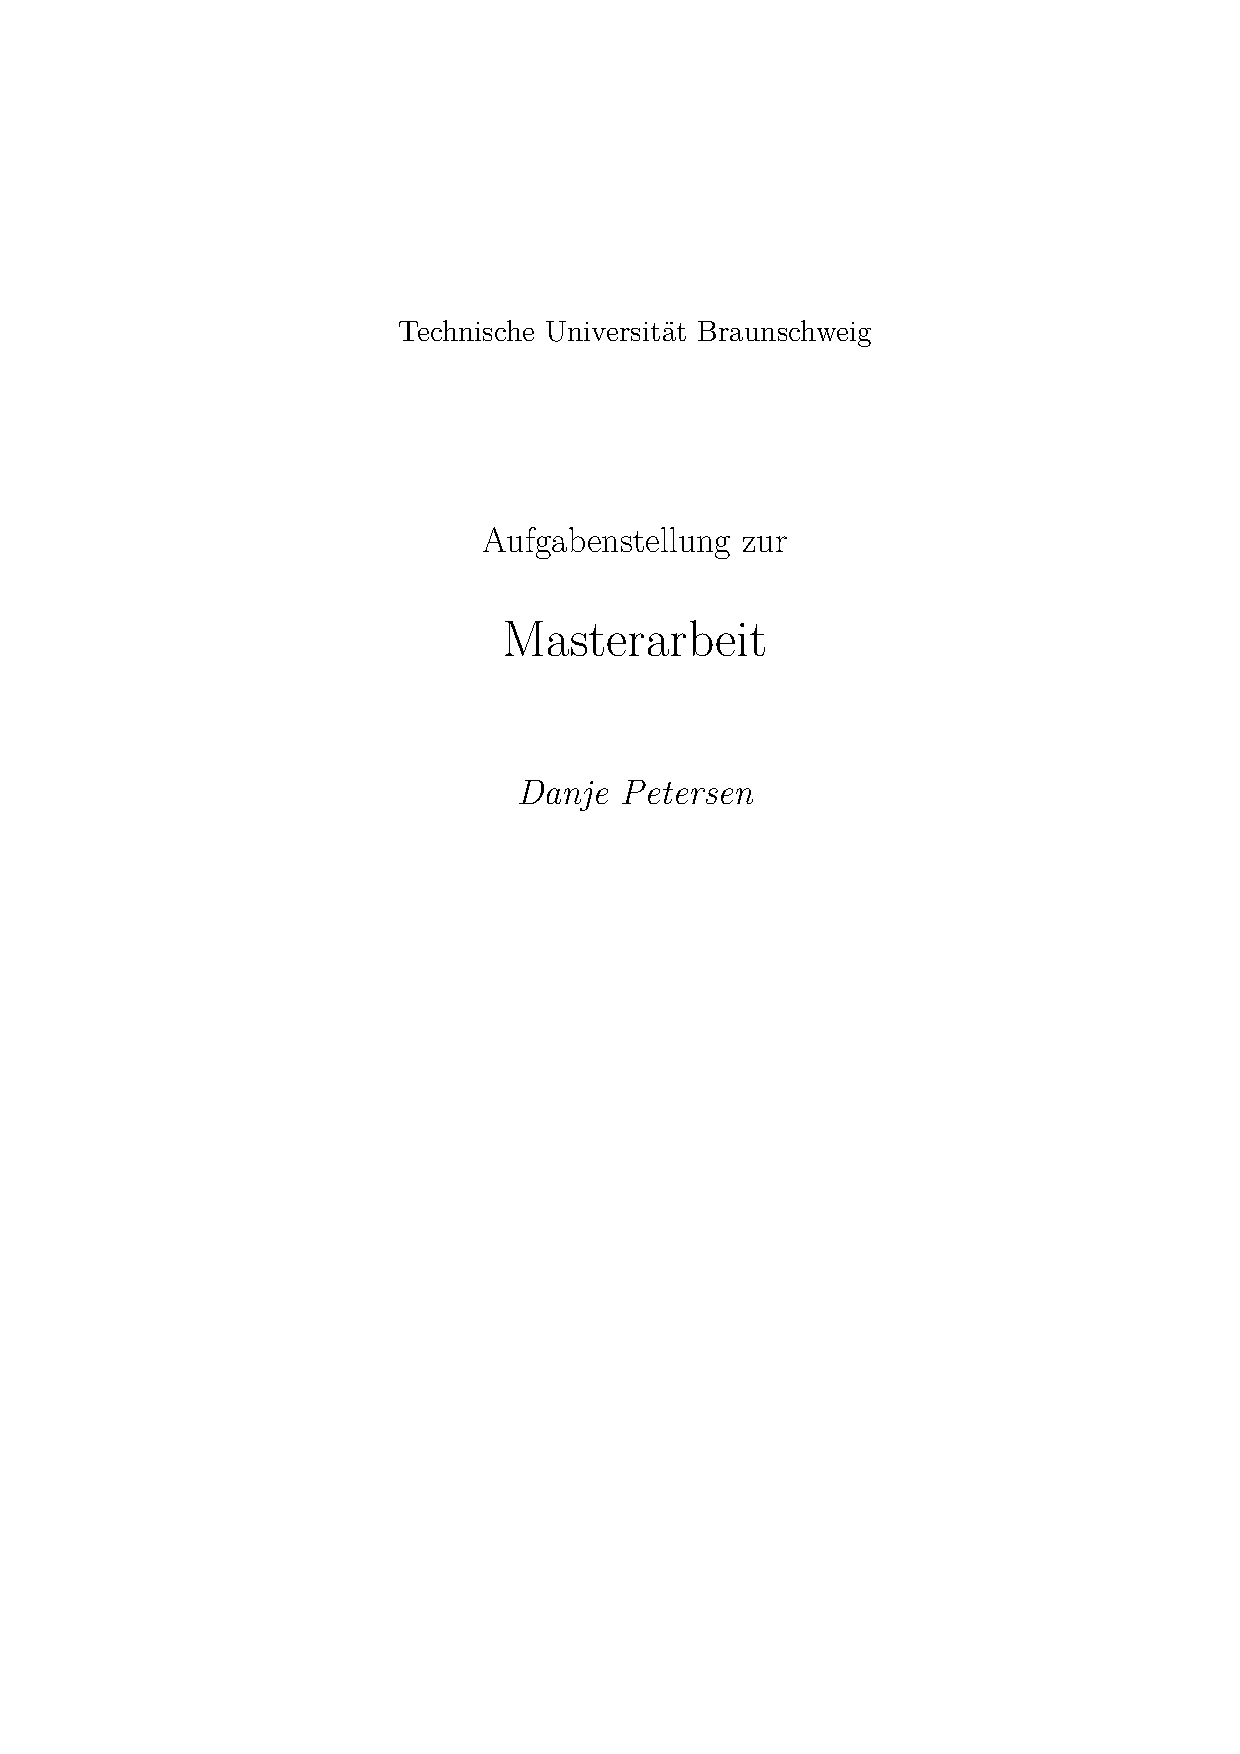
\includepdf{includes/Titelseite/build/title.pdf}

\title{Task for the Master's Thesis}
\author{Danje Petersen}

\maketitle
%\noindent \begin{Huge}\textbf{Aufgabenstellung zur Masterarbeit}\end{Huge} \\
%Danje Petersen


\section{Motivation}
Modern computers come with a set of processors that can run simultaneously. To utilize this for their advantage, developers started to design their programs to use multiple concurrently running threads.
Since these threads might still operate on the same memory it is possible to encounter problems like data-races when executing these programs. Data races occur when two or more threads access the same memory space and at least one of them uses a write operation.
The classic example is the following: \\

\begin{figure}[h]\label{example}
\centering
\begin{tabular}{c||c}
\multicolumn{2}{c}{\texttt{Init:x=y=0;}} \\[4mm]
%Thread 1: & Thread 2:\\[4mm]

\texttt{x=1;} & \texttt{y=1;} \\
\texttt{a=y;} & \texttt{b=x;} \\
\end{tabular}
\caption{Example of two threads using the same variables. Depending on how the threads are scheduled, the resulting values could feature any combination of $1$ and $0$ for the variables $a$ and $b$.}
\end{figure}

Since this might lead to inconsistent results and therefore unpredictable behaviour, programming languages and cpu architectures provide memory consistency models. If the developer confines themselves to these rules, they get certain guarantees in return. 
These memory consistency models describe how threads are allowed to interact with each other when it comes to shared memory. 

\todo{Warum ist es wichtig die Modelle zu verifizieren?}

\section{Current Research}

\todo{Einordnung in ein weiter gefasstes Feld von Memory Consistency} \\

\todo{Fragen die sich in diesem Forschungsfeld stellen (siehe Kater paper)}\\

\todo{was bedeutet "weak" memory?} \\
In 2014 Alglave et al. proposed an axiomatic framework for modelling weak memory and the corresponding language CAT \cite{Alg+14}. Axiomatic models work by constraining relations on memory access.

\begin{figure}[h]
\begin{align*}
\langle cat\rangle &:= \langle constraint\rangle \mid \langle cat \rangle~ \langle cat\rangle \\
\langle constraint \rangle &:= \texttt{acyclic } \langle rel \rangle \mid \texttt{irreflexive } \langle rel \rangle \\
\langle rel \rangle &:= \langle base\_rel \rangle \mid \langle rel \rangle . \bangle{rel} \mid \bangle{rel}^* \mid \bangle{rel} \cup \bangle{rel} \mid \bangle{rel} \cap \bangle{rel} \\ &\quad \mid \bangle{rel}^{-1} \mid \bangle{rel}^+ \mid \bangle{rel}? \mid \bangle{base\_set} \times \bangle{base\_set} \mid \textcolor{red}{\bangle{rel}\setminus \bangle{rel} \mid{} \sim\bangle{rel}} \\
\bangle{base\_rel} &:= \text{po} \mid \text{rf} \mid \text{rmw} \mid \text{loc} \mid \text{ext} \mid \text{id} \mid \emptyset \\
\bangle{base\_set} &:= \text{R} \mid \text{W} \mid \text{F} \mid \text{B} \mid \text{M} \mid \text{IW} \mid \text{E}
\end{align*}
\caption{The CAT language when including the red coloured terms, when excluding them it is the fragment called rational CAT. $\bangle{rel}^+$ is the transitive closure, $\bangle{rel}?$ the reflexive closure, $\bangle{rel}^*$ the reflexive and transitive closure, $\sim\bangle{rel}$ the complement \cite{Alg+14}.}   
\label{cat}
\end{figure}

Some very basic examples for these relations are the \textit{program order} (po) which represents the sequence of events of a single thread and \textit{read-from} (rf), displaying for every read which write determined the value it sees. Upon these and some more base relations, memory consistency models can be expressed with CAT as can be seen in \cref{cat}.

While the tool that Alglave et al. developed allows to test certain programs in a given memory model, verifying these models is a different issue. Verification of the memory consistency model means checking if a given model guarantees certain properties for every program that can be executed under it. The first tool to tackle this issue was KATER \cite{Kok+23} which covered only a fragment of CAT that could be transformed into Kleene algebra with tests. This fragment excluded set difference, complement, intersections, converses and the construction of relations from sets. \\
The next year Koutsouridis et al. presented KATI \cite{Kou+24} which is able to handle converses and some intersections.

The first tool that addressed all intersections as well as inverses and construction of relations from sets (called rational CAT, see \cref{cat}) was developed by the supervisors of this master's thesis in 2025 \cite{GruMey25}. In their yet to be published work, they presented a logical theory of relations where the unsatisfiability of a formula is equivalent to the model fulfilling a condition. The formula consists of a negated subformula representing the memory model and a subformula for the condition. \\
The formula is then decomposed until there exists a program execution that fulfills it or it is determined unsatisfiable.


\section{Task}
The decomposition used in \cite{GruMey25} might result in infinite paths when unrolling Kleene stars. This leads to the authors using a cyclic proof system that returns to a node in the decomposition tree when it is equal to the current node.
The task for this master's thesis is to replace this cyclic proof system with one that uses invariants and is neither cyclic nor infinite. Additionally the new proof system is supposed to directly handle inclusion between memory models and does not need to resolve them to the event level.
The student is supposed to create a proof system that works reasonably well and ideally proof it's completeness and soundness. 


\printbibliography

\end{document}

